\documentclass[11pt]{beamer}
\usetheme{Darmstadt}
\useoutertheme{split}
\useoutertheme{miniframes}
\usepackage{hyperref}
\usepackage{bm}
\usepackage{times}
\usefonttheme{structurebold}
\usepackage{array}
\usepackage[english]{babel}
\usepackage{amsmath,amssymb,amsthm,mathrsfs,amsfonts,dsfont}
\usepackage[latin1]{inputenc}
\usepackage{adjustbox}
\usepackage{graphicx}
%Code snippets and syntax highlighting
\usepackage{listings}
%Settings for Listings
\lstset{
  language=Python,
  basicstyle=\ttfamily,
  keywordstyle=\color{blue}\ttfamily,
  stringstyle=\color{red}\ttfamily,
  commentstyle=\color{green}\ttfamily,
  morecomment=[l][\color{magenta}]{\#}
}

\usepackage{array}
\usepackage{threeparttable}
\usepackage{booktabs}
\usepackage{colortbl}
\usepackage{multirow}
\usepackage{amsthm}
\usepackage{float,graphicx,color}
\newtheorem*{thm}{Theorem}
\theoremstyle{definition}
%\numberwithin{equation}{section}
\newtheorem*{defn}{Definition}
\newcommand\boldline{\arrayrulewidth{1pt}\hline}
\newcommand\ve{\varepsilon}


\setbeamercovered{dynamic}

\title[Econ 741 Project]{PAYG, Current Account and Fertility Rates: \\ Consequences for Savings}
\author[Clawson]{Jeff Clawson}
\date{\today}


\begin{document}

\begin{frame}
\titlepage % Print the title page as the first slide
\end{frame}

\begin{frame}
\frametitle{Overview} % Table of contents slide, comment this block out to remove it
%\tableofcontents % Throughout your presentation, if you choose to use \section{} and \subsection{} commands, these will automatically be printed on this slide as an overview of your presentation
\begin{itemize}
    \item Motivating Graphs

    \item Quick Literature Review

    \item Endgame Model

    \item Current Model

    \item Steady State Calculations

\end{itemize}
\end{frame}

%----------------------------------------------------------------------------------------
%	PRESENTATION SLIDES
%----------------------------------------------------------------------------------------


%------------------------------------------------
\section{Motivation} 
%------------------------------------------------
\begin{frame}
    \frametitle{US Budget}
\begin{figure}
	\centering
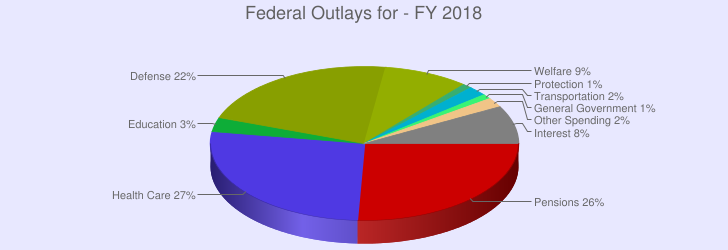
\includegraphics[scale=0.5]{chart.png}
	\label{V1}
\end{figure}

\end{frame}




\begin{frame}
    \frametitle{Japan Budget}
\begin{figure}
	\centering
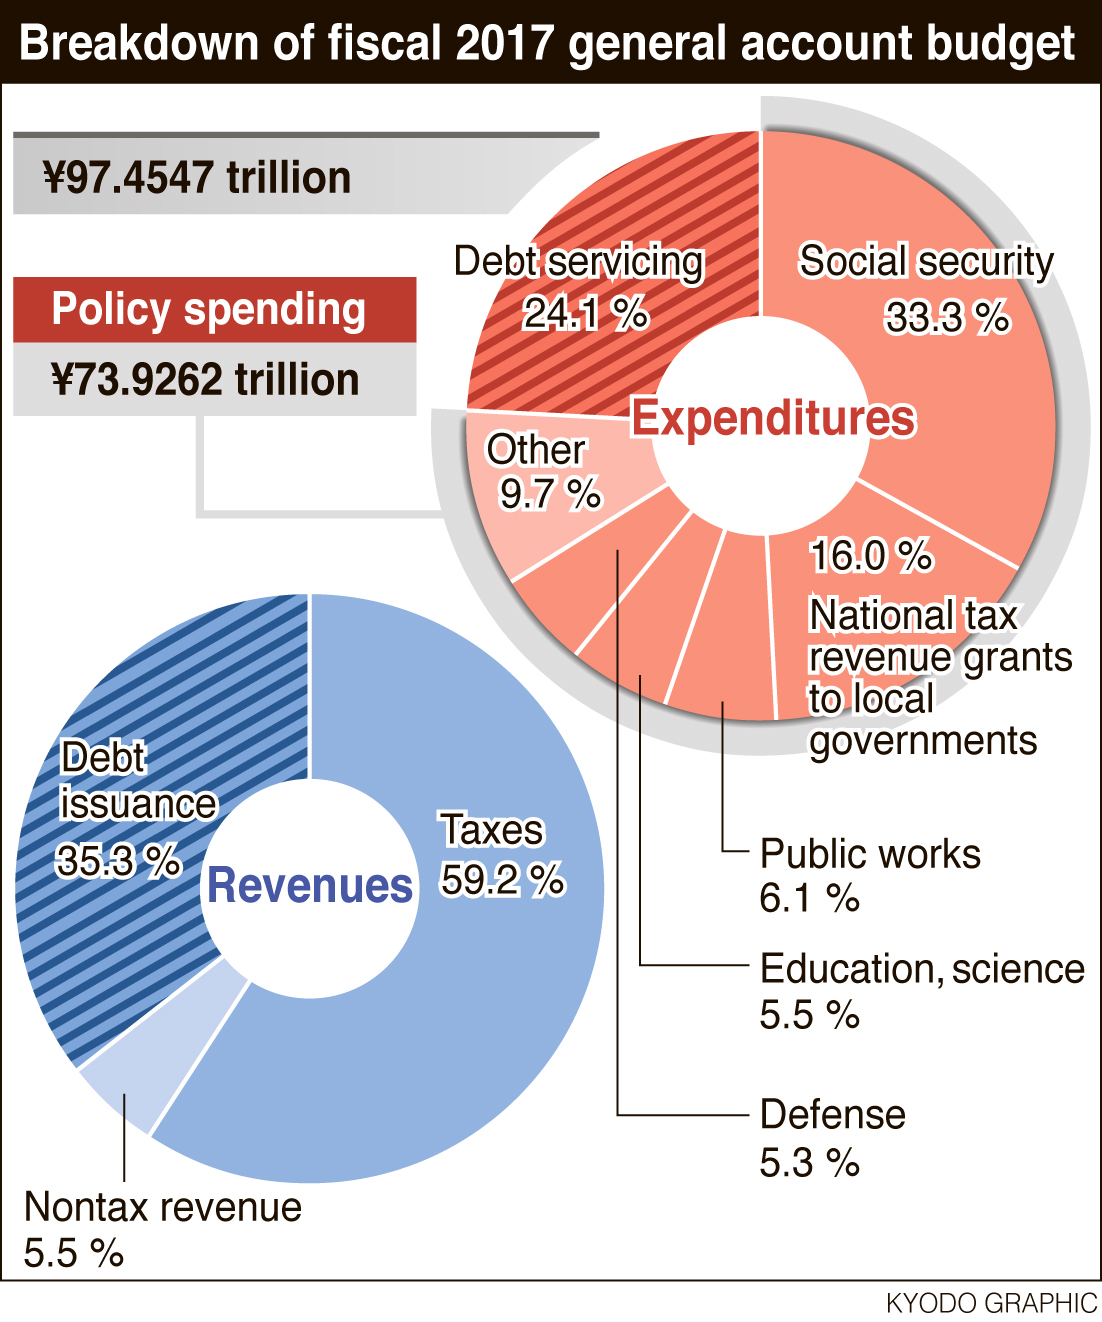
\includegraphics[scale=0.5]{japan_budget.jpg}
	\label{V2}
\end{figure}

\end{frame}


\begin{frame}
    \frametitle{Government Debt and Fertility}
\begin{figure}
	\centering
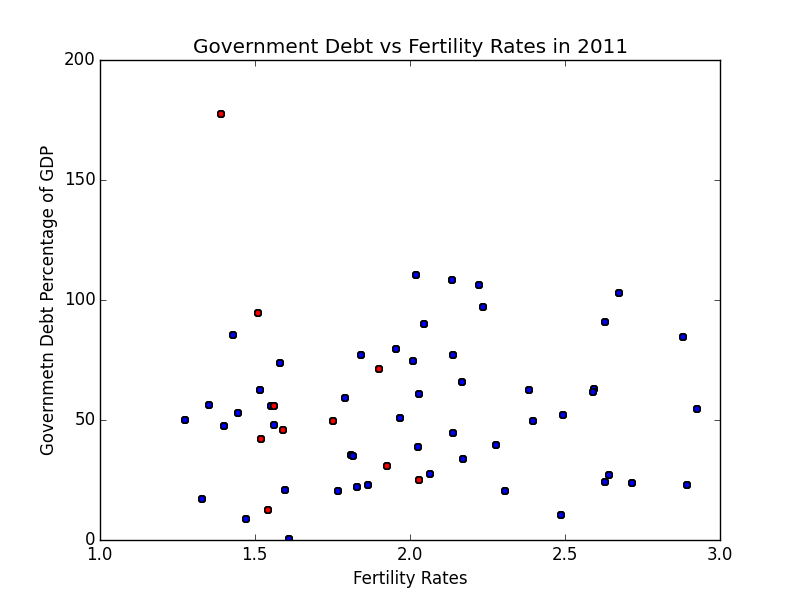
\includegraphics[scale=0.5]{Debt_Fert.png}
	\label{V3}
\end{figure}

\end{frame}



\begin{frame}
    \frametitle{Current Account and Fertility}
\begin{figure}
	\centering
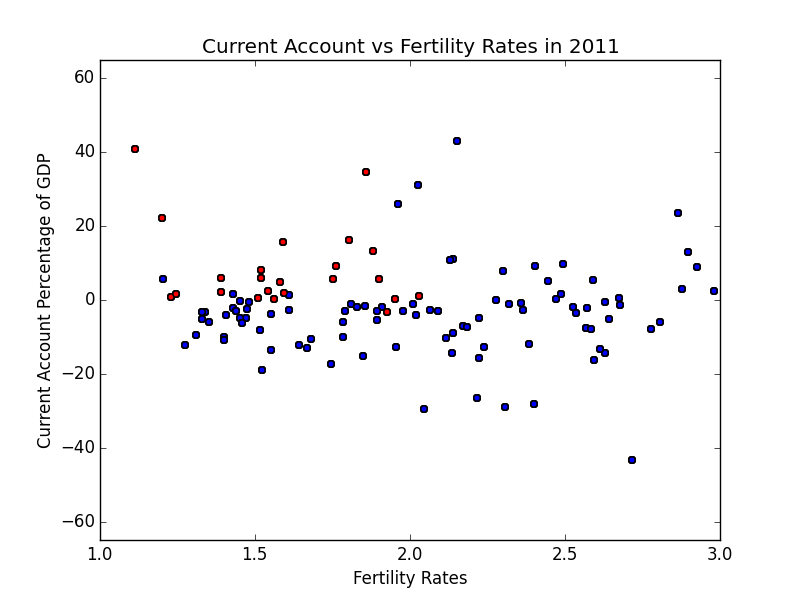
\includegraphics[scale=0.5]{CA_Fert.png}
	\label{V4}
\end{figure}

\end{frame}

\begin{frame}
    \frametitle{Underlying Question}

    \begin{itemize}
        \item What is the impact of a Pay-As-You-Go Pension System and a shrinking population on international financial allocation?
        \item I will begin this exploration by building a model. This will be an overlapping generations model (OLG).

    \end{itemize}


\end{frame}

%------------------------------------------------
\section{Lit Review} 
%------------------------------------------------
\begin{frame}
    \frametitle{A Brief Review}

    \begin{itemize}
        \item \textbf{OLG in International Trade/Finance}
            \begin{itemize}
                \item Stavely-O'Carroll and Stavely-O'Carroll (2017): Comparing two countries with and without PAYG system.

                \item Eugeni (2015): Differences in PAYG execution lead to impact on current accounts
                \item Sayan (2005): Two Countries growing at different rates


            \end{itemize}

        \item \textbf{OLG/Pension and Saving}
            \begin{itemize}
                \item Samwick (2000): Pension system's impact on savings, Empirical

            \end{itemize}

    \end{itemize}

\end{frame}

%------------------------------------------------
\section{Ideal Model} 
%------------------------------------------------
\begin{frame}
    \frametitle{Unique Features}
I am working to build a two good, two country OLG Trade Model with the following features:
    \begin{itemize}
        \item Both countries have a Pay-As-You-Go (PAYG) pension system and exhibit population growth.
        \item However, one will have stochastic population growth and the other will grow at a constant rate.
        \item The governments will be permitted to borrow to finance pensions
        \item Households can purchase good from either firms. They could be subject to trade costs.

    \end{itemize}


\end{frame}



\begin{frame}
    \frametitle{Ideally..}
\frametitle{Full Model Diagram}
\begin{figure}
	\centering
	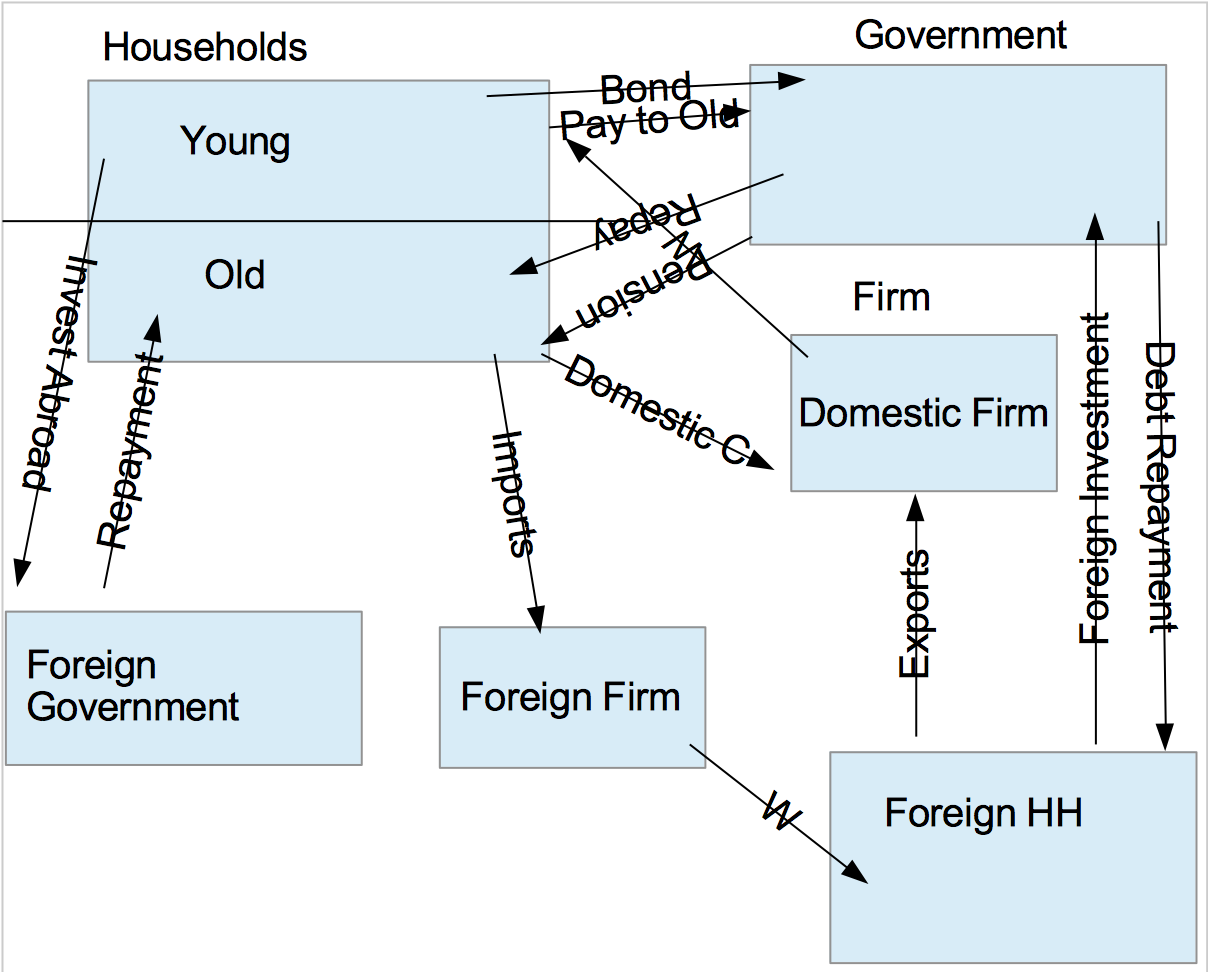
\includegraphics[scale=0.35]{Full_Model.png}
	\label{V5}
\end{figure}
\end{frame}

%------------------------------------------------
\section{Current Model} 
%------------------------------------------------
\begin{frame}
    \frametitle{Starting from the Ground Up (Households)}
    First, I'll focus on the stochastic population mechanic before adding the other features. The Household's problem is:
    \[\max_{s_t,c_t^y,c_{t+1}^o} u(c_t^y)+\beta \mathds{E}_t u(c_{t+1}^o)\]
    \[c_t^y = w_t - x_t - s_t\]
    \[c_{t+1}^o = p_{t+1} + (1+r_{t+1}) s_t\]
    Where the population grows:
    \[N_t = (1+g_t e^{z_t}) N_{t-1}\]
    Where $z_t = \rho z_{t-1} + \epsilon_t \text{   }\epsilon_t \sim N(0,\sigma_t^2)$


\end{frame}

\begin{frame}
    \frametitle{Firm and Government}
    Pensions must equal contributions
    \[N_t x_t = N_{t-1} p_t \implies p_t = (1+e^{z_t}g_t)x_t\]
    Then the firm's problem is:
    \[\max_{k_t} k_t^\alpha -w_t -r_t k_t\]
    With the standard factor prices:
    \[r_t = \alpha k_t^{\alpha-1}\]
    \[w_t = f(k_t) - k_t f'(k_t)\]

\end{frame}

\begin{frame}
    \frametitle{Equilibrium Conditions}
    Given (Assuming CRRA utility) factor prices $(w_t,r_t)$, $x_t$ and $k_t$ satisfy:
    \[(c_t^y)^{-\sigma}=\beta \mathds{E}_t(1+r_{t+1})(c_{t+1}^o)^{-\sigma}\]
    \[k_t^\alpha = c_t^y + c_{t}^o + k_t +x_t\]
    Using the constraints defined before.

\end{frame}

%------------------------------------------------
\section{Steady State} 
%------------------------------------------------
\begin{frame}
    \frametitle{"Calibrations"}
    \begin{table}
\begin{tabular}{lr}
\toprule
{Parameter} & Value \\
\midrule
$g$  &  .03 \\
$\beta$  &  .95 \\
$\alpha$  &  .35 \\
$\delta$  &  .04 \\
\bottomrule
\end{tabular}
\end{table}

\end{frame}

\begin{frame}
    \frametitle{"Results"}
    $k_{ss}$:  0.0108942393752\\
    $x_{ss}$:  0.0521844807871\\
    $r_{ss}$:  6.60526202666\\
    $w_{ss}$:  0.133638710501\\
    $c^y_{ss}$:  0.0705599903384\\
    $c^o_{ss}$:  0.13660356024


\end{frame}





%------------------------------------------------
\section{Next Steps\dots} 
%------------------------------------------------
\begin{frame}
    \frametitle{Next Stage}
    \begin{itemize}
        \item Need to figure Constraint with the $c_t^o$
        \item Next, I'll incorporate bond markets.
        \item Then, I'll add trade.
    \end{itemize}

\end{frame}

%\begin{frame}
%\frametitle{Value Function, Original Grid}
%\begin{figure}
%	\centering
%	\includegraphics[scale=0.5]{V1.jpg}
%	\label{V1}
%\end{figure}
%\end{frame}


%----------------------------------------------------------------------------------------

\end{document}
